\chapter {Diseño}

\section{Solución adoptada}
        \begin{text}
                Con el fin de cumplir todos los objetivos definidos en la sección \nameref{objetivos_primarios} se han elegido las siguientes tecnologías. Cabe destacar la influencia ejercida por la empresa para utilizar tecnologías ya existentes en la infraestructura actual como los firewall pfSense o el servicio de virtualización Proxmox. Sin embargo, son tecnologías con continuo desarrollo y muy aptas para desarrollar su papel dentro del cluster. \\
                Todas las tecnologías que se van a mencionar a continuación son de código abierto y satisfacen las necesidades de este proyecto. 
        \end{text}

        \subsection{Proveedor Infraestructura}
                \begin{text}
                        La infraestructura necesaria para formar el ecosistema que cumpla con los objetivos de este proyecto, se ha de alojar en servidores físicos. Para cumplir esta necesidad se ha elegido el proveedor Hetzner \cite{hetzner:online}, uno de los proveedores de servidores bare metal más conocidos en Europa. \\
                \end{text}
                 \clearpage
                \subsubsection{Hetzner}
                \begin{text}
                        Hetzner posee tres grandes centros de datos, Suiza, Irlanda y Luxemburgo. Una de las principales ventajas que tiene Hetzner sobre otras compañías es el soporte 24/7 que ofrece en los servidores dedicados. Ante cualquier problema siempre tienes una línea abierta de soporte para solucionarlo. Esto junto con la gran variedad de servidores de distintas gamas que ofrece, hace a Hetzner un candidato perfecto para contratar la infraestructura.

                        \begin{figure}[!hbt]
                                \centering
                                \includegraphics[scale=0.75]{imagenes/Diseno/baremetal.jpeg}
                                \caption[Hetzner Data Center]{Hetzner Data Center \cite{hetzner:online}} 
                                \label{Hetzner Data Center}
                        \end{figure} 

                        \begin{figure}[!hbt]
                                \centering
                                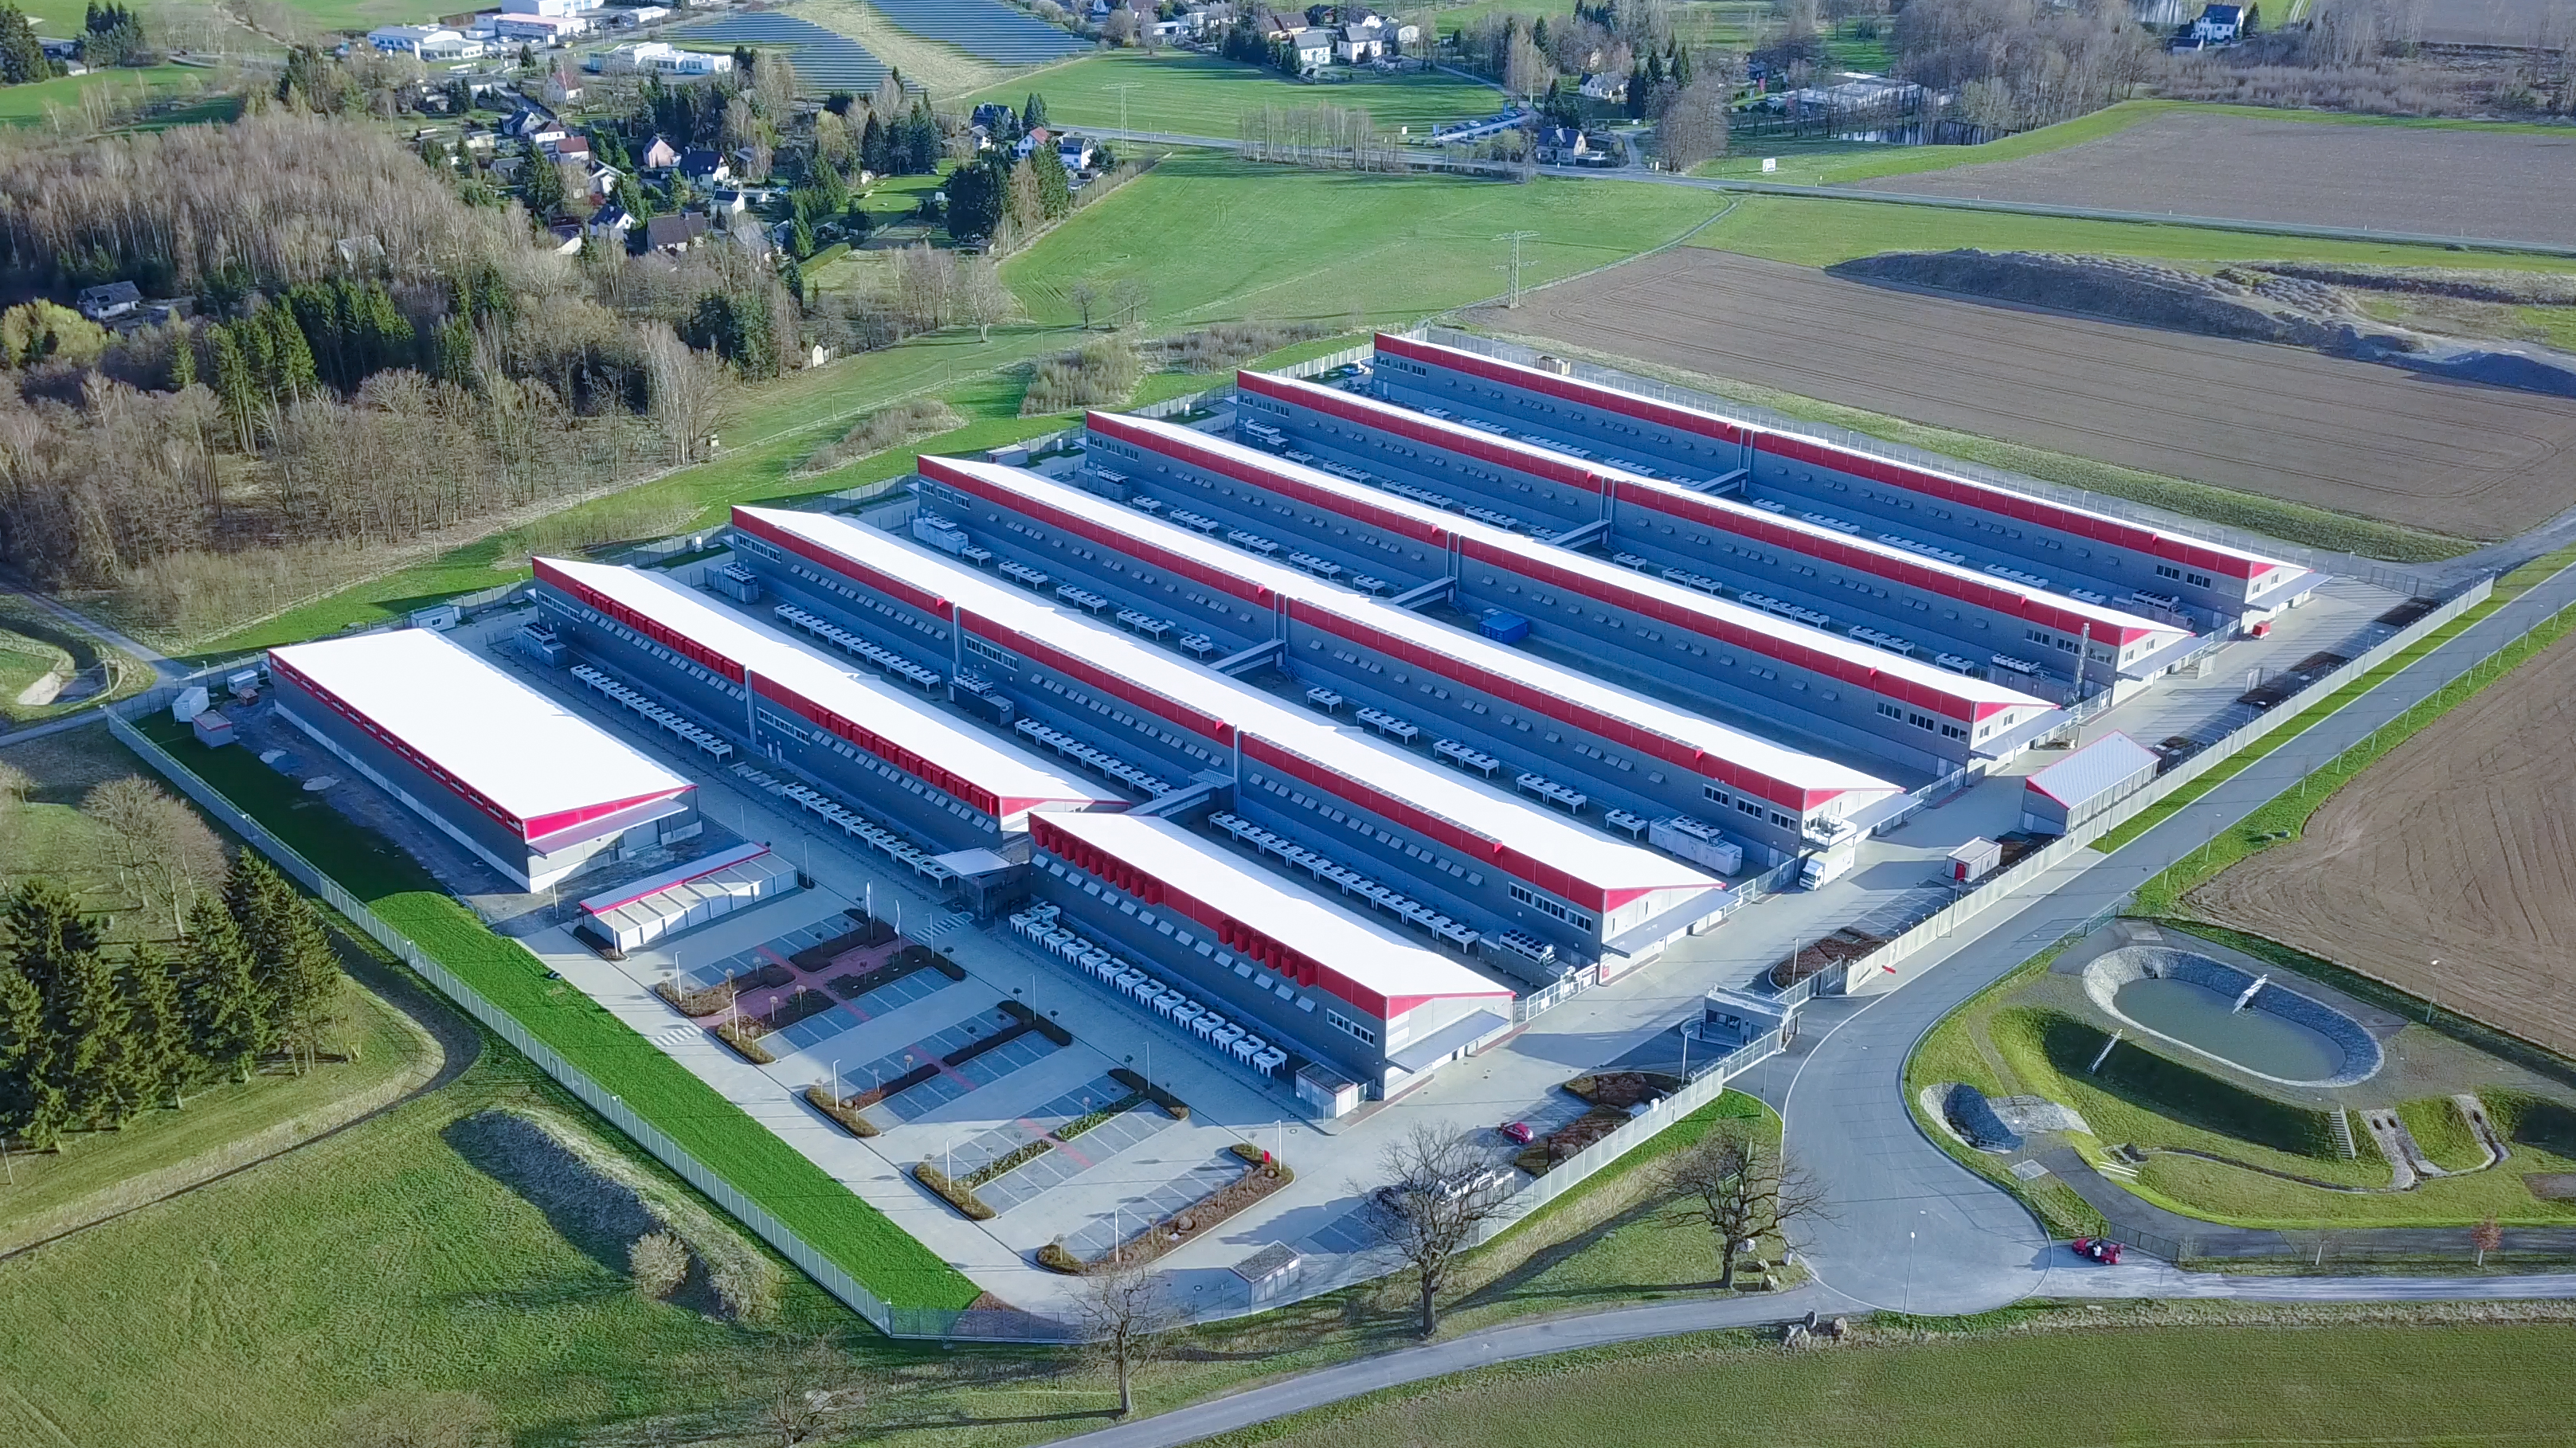
\includegraphics[scale=0.5]{imagenes/Diseno/datacenter.jpg}
                                \caption[Hetzner Building]{Hetzner Building \cite{hetzner:online}} 
                                \label{Hetzner Building}
                                \end{figure} 
                        \end{text}

        \subsection{Servicio Virtualización}
                \begin{text}
                        Para poder ofrecer todos los servicios descritos en \nameref{objetivos_primarios} y cumplir con la arquitectura objetivo \nameref{Infraestructura_objetivo}, se hace necesario añadir una capa de virtualización a los servidores contratados. Estos 3 servidores físicos, servirán para desplegar los servicios descritos, sin embargo es necesario separar estos servicios en distintas máquinas. El servicio de virtualización nos permitirá crear tantas máquinas virtuales como servicios, virtualizando el hardware del servidor físico y aportando entornos cerrados, virtualizados y fácilmente recreables. \\
                        El servicio de virtualización elegido ha sido Proxmox VE \cite{proxmox:online}, basado en KVM (Kernel-based Virtual Machine) y de código abierto. Se ha elegido este servicio de virtualización por necesidades de la empresa.
                \end{text}
                \subsubsection{Proxmox}
                \begin{text}
                        Proxmox VE es una solución completa para gestionar máquinas virtuales KVM. Entre sus servicios podemos destacar:
                        \begin{itemize}
                                \item \textbf{Hypervisor KVM}. Fácil acceso a las máquinas a través de una consola gestionada por el hypervisor KVM.
                                \item \textbf{ISO}. Creación y gestión de máquinas virtuales tanto Windows como Linux.
                                \item \textbf{Storage}. Software-defined storage. Podemos crear soluciones de almacenamiento con posibilidad de integrar tecnologías como CEPH o glusterfs.
                                \item \textbf{Networking}. Solución a la gestión de redes desde un punto de vista software. Se pueden crear tantas interfaces virtuales como se necesiten.
                                \item \textbf{Backups}. Gestión de backups completo de las máquinas.
                                \item \textbf{User management}. Gestión de espacios de usuario así como restricción de permisos según tipo de usuario.
                                \item \textbf{Firewall}. Firewall por máquina virtual y por cluster. El firewall se puede manejar por la interfaz web o por la API.
                                \item \textbf{Proxmox VE API}. La interfaz web es una gran ayuda para el Administrador, sin embargo Proxmox también posee una extensa API \cite{ProxmoxAPI:online} para poder realizar todo lo que se puede hacer desde la interfaz web, desde línea de comandos a través de su API con el comando \textbf{pvesh}
                                \item \textbf{Proxmox Forums}. Al no ser la versión enterprise, Proxmox VE no dispone de soporte dedicado como tal, sin embargo posee una gran comunidad muy activa que responden a tus dudas en los foros \cite{ProxmoxForum:online}.
                                \item \textbf{Interfaz Web.} Gracias a su interfaz web, se hace muy sencilla la gestión de las distintas máquinas.
                                \begin{figure}[!hbt]
                                        \centering
                                        \includegraphics[scale=0.355]{imagenes/Diseno/proxmox_wui.png}
                                        \caption[Proxmox WUI]{Proxmox WUI} 
                                        \label{Proxmox WUI}
                                \end{figure}
                        \end{itemize}
 
                \end{text}
        \subsection{Firewall}
                \begin{text}
                        Hoy en día, con el auge de la informática y de las nuevas tecnologías, cada vez se están dando más y más ciberataques. Los denominados 'hackers' o delincuentes, aprovechan brechas de seguridad en los sistemas para poder hacerse con información sensible y después poder pedir rescate por dicha información. Estos ataques suelen aprovechar puertos abiertos, servicios obsoletos y vulnerabilidades conocidas para perpetrar sus ataques. Por ejemplo, esta web nos muestra en tiempo real la cantidad de ataques que sufre un país determinado \cite{ciberataques:online}.
                        \begin{figure}[!hbt]
                                \centering
                                \includegraphics[scale=0.3]{imagenes/Diseno/ciberataques.png}
                                \caption[Ciberataques]{Ciberataques \cite{ciberataques:online}} 
                                \label{Ciberataques}
                        \end{figure}
                        Es por esto que se hace necesaria la protección de la infraestructura final, exponiendo únicamente los puertos necesarios para desviar el tráfico y trabajar con los servicios únicamente dentro de la red LAN segura. \\
                        Para este fin se ha elegido la tecnología pfSense \cite{pfsense:online}. PfSense dispone de su versión community gratuita y de código abierto. Esta tecnología se ha elegido ya que es la tecnología utilizada en el cluster de producción de la empresa.
                \end{text}

                \subsubsection{pfSense}
                        \begin{text}
                                Basado en FreeBSD, este firewall se instala en una máquina virtual como un servicio más sirviendo como router/firewall según la configuración. Entre otros, los principales servicios que ofrecen pfSense son:
                                \begin{itemize}
                                        \item \textbf{DHCP Server}. Un servidor DHCP totalmente configurable para asignar ya sea de forma dinámica o estática las IP a las máquinas del cluster.
                                        \item \textbf{DNS Resolver}. Posibilidad de configurar el servidor DNS. Forzar resolución de nombres, modificar servidores...
                                        \item \textbf{Firewall}. Por defecto deniega todo el tráfico menos el necesario para la interfaz web. Podemos definir reglas firewall dedicadas para cada interfaz. También podemos crear reglas NAT para redirigir el tráfico dentro de la red. Todo gestionado desde la interfaz web.
                                        \item \textbf{Virtual IP}. Al querer ofrecer alta disponibilidad, es necesario disponer de una ip virtual del tipo CARP (Common Address Redundancy Protocol). De esta forma podemos tener una IP virtual de acceso al cluster para los firewall. En caso de fallo del firewall principal, se modificará esta IP para que el pfSense secundario se haga cargo de dirigir el tráfico dentro del cluster a través de esta ip virtual.
                                        \item \textbf{Interfaces}. Creación y asignación de interfaces. A través de la interfaz de usuario o dentro de la propia consola de la máquina virtual, podemos definir las distintas interfaces necesarias, asignarles ip y asociarlas con interfaces físicas del anfitrión.
                                        \item \textbf{Package Manager}. La interfaz web posee un gestor de paquetes muy útil que nos ofrece una gran variedad de paquetes que nos facilitarán el uso de pfSense. Paquetes como tinc, openvpn, HAproxy que no vienen integrados por defecto en pfSense pero se pueden añadir gracias a este gestor de paquetes.
                                        \item \textbf{VPN}. Gestión de redes VPN para realizar conexiones con equipos fuera del cluster. Por ejemplo esto ha resultado muy útil para poder conectar el equipo de desarrollo con las distintas máquinas virtuales del cluster a través de una VPN. Esto nos permite no exponer ningún puerto y poder tener acceso.
                                        \item \textbf{Services Status}. Dentro de la interfaz web, disponemos de un panel informativo con el estado de cada uno de los servicios gestionados por pfSense. A través de este pequeño panel de control, podemos comprobar el estado, reiniciar o parar un servicio.
                                        \item \textbf{Web Interface}. Esta es la parte más atractiva de pfSense, ya que podemos configurarlo de una forma intuitiva y a través de una interfaz web.
                                        \begin{figure}[!hbt]
                                                \centering
                                                \includegraphics[scale=0.3]{imagenes/Diseno/pfsense_wui.png}
                                                \caption[pfSense interfaz web]{pfSense interfaz web} 
                                                \label{pfsense_wui}
                                        \end{figure}
                                \end{itemize}
                        \end{text}
                \clearpage
        \subsection{Contenedores}
                \begin{text}
                        Como ya hemos visto, Proxmox nos proporciona una capa de virtualización del hardware de los servidores para poder crear máquinas virtuales donde alojar los distintos servicios. \\
                        Sin embargo, a la hora del desarrollo y despliegue de aplicaciones web en el cluster, se hace inviable crear una máquina virtual por cada una de las aplicaciones web creadas. Esto sería insostenible ya que las máquinas virtuales demandan recursos. \\

                        Para solventar este problema se van a crear aplicaciones en contenedores. Cada aplicación tendrá uno o varios contenedores dependiendo de los servicios, normalmente 1 servicio 1 contenedor. Para realizar este proceso se ha elegido la tecnología Docker. \cite{docker:online}.
                \end{text}
                \subsubsection{Docker}
                \begin{text}
                        Docker es la tecnología más famosa para crear contenedores. Gracias a Docker podemos aislar las aplicaciones en contenedores seguros y fácilmente replicables. Se ha elegido Docker por su extensa comunidad y porque es la tecnología más utilizada para este fin. Sin embargo, con esto no es suficiente ya que, una vez tengamos la aplicación separada en contenedores, necesitamos un entorno donde lanzar estos contenedores y poder gestionarlos. Es aquí donde surgen los orquestadores de contenedores. A continuación se hace una pequeña a dos orquestadores: Docker Swarm \cite{swarm:online} y Kubernetes \cite{k8:online}.
                \end{text}
        \subsection{Orquestación contenedores}
                \subsubsection{Kubernetes}
                \begin{text}
                        Kubernetes es un software de orquestación de contenedores que nos permite automatizar el proceso de despliegue, escalado y gestión de las aplicaciones en contenedores. Kubernetes se ha convertido en la solución principal para grandes empresas por su robustez. La principal ventaja de Kubernetes frente a sus competidores es la posibilidad de modificar las condiciones de escalado vertical o horizontal de los contenedores sin afectar a la disponibilidad de la aplicación. Su gran desventaja es la complejidad, ya que para poder manejar de forma eficiente un cluster de Kubernetes debemos pasar por un largo camino de aprendizaje. \\
                        Se ha elegido esta tecnología por su gran demanda en el sector y como proceso de aprendizaje. Esta tecnología no estaba implementada en la empresa, sin embargo, se va a introducir como orquestador adicional.
                \end{text}
                \subsubsection{Docker Swarm}
                \begin{text}
                        Docker Swarm es un software de orquestación de contenedores. Es la solución nativa de Docker para la gestión de los contenedores. Docker Swarm nos permite automatizar los procesos de despliegue escalado y gestión de contenedores. Sin embargo, cuando hablamos de escalado vertical o horizontal, Docker Swarm, al contrario que Kubernetes, no permite este escalado asegurando la disponibilidad. Debemos relanzar los contenedores con los nuevos parámetros para el escalado. \\
                        Se ha elegido esta tecnología por ser la usada en un principio en la empresa para la gestión de contenedores. Cabe destacar que, aunque no ofrece los mismos servicios que Kubernetes, Docker Swarm es una solución muy buena para la orquestación de contenedores y su principal ventaja frente a Kubernetes es la facilidad para desplegar y gestionar los contenedores.
                \end{text}
        \subsection{Almacenamiento estático}
                \label{ceph}
                \begin{text}
                        Si bien tanto Docker Swarm como Kubernetes nos permiten gestionar los contenedores, estas tecnologías están pensadas para aplicaciones stateless o sin estado \cite{stateless:online}. A grandes rasgos, esto quiere decir que tanto Kubernetes como Docker Swarm, funcionan bien con aplicaciones que no necesitan almacenar información para su correcto funcionamiento. \\
                        Para esto, Docker ofrece una solución en forma de volúmenes. Sin embargo, esta solución no se adecua a las necesidades de un entorno de alta disponibilidad  y alta fiabilidad. Es por esto que surge la necesidad de crear alguna solución de almacenamiento distribuido que nos proporcione dichas características. La solución elegida ha sido Ceph \cite{ceph:online}.
                \end{text}
                \subsubsection{Ceph}
                \begin{text}
                        Ceph es un software de código abierto que proporciona almacenamiento distribuido. Ceph ofrece almacenamiento a nivel de bloque, objeto y a nivel de fichero. \\
                        En nuestro caso particular, nos vamos a beneficiar de CephFS o Ceph File System, que está implementado sobre el sistema de almacenamiento a nivel de bloque creado por Ceph. Las principales ventajas de Ceph son:
                        \begin{itemize}
                                \item Seguridad de la información
                                \item Almacenamiento ilimitado por sistema de ficheros.
                                \item Balanceo de carga.
                                \item Alta disponibilidad y alta fiabilidad.
                                \item Interfaz web. Ceph nos ofrece la opción de gestionar el cluster desde una interfaz web. Aunque las opciones son limitadas ya que está bajo desarrollo, facilita en gran medida la gestión del cluster.

                                \begin{figure}[!hbt]
                                        \centering
                                        \includegraphics[scale=0.35]{imagenes/Diseno/ceph_wui.png}
                                        \caption[CEPH interfaz web]{CEPH interfaz web} 
                                        \label{ceph_wui}
                                \end{figure}
                        \end{itemize}

                        Se ha elegido esta tecnología por ser la más completa de las opciones de código abierto. 

                \end{text}

        \subsubsection{Aclaraciones Ceph}
        \label{cephdefinitions}
        \begin{text}
                Ceph es una tecnología compleja, para abordar de forma correcta este documento se cree necesaria la aclaración de cómo funciona Ceph así como de los servicios que involucra:


        \end{text}
        \subsection{Servidor Web / Proxy}
                \begin{text}
                        Para el correcto acceso de los clientes y desarrolladores a las aplicaciones, se hace necesario un proxy que desvíe las peticiones a la aplicación correcta. Para este fin se ha elegido la tecnología Nginx \cite{nginx:online}, que sirve a la vez de servidor web y de proxy. Un proxy es esencial para asegurar la seguridad del cluster, ya que únicamente hay un punto de entrada protegido por un proxy que a su vez está protegido por el firewall. De esta forma se aumenta la seguridad y se dificultan los intentos de ataque masivos.
                \end{text}
        \clearpage
                \subsubsection{Nginx}
                \begin{text}
                        Nginx, es uno de los servidores web más utilizados en el mundo por su facilidad en el uso así por su versatilidad, puede ser utilizado como servidor web, proxy o balanceador. 

                        \begin{figure}[!hbt]
                                \centering
                                \includegraphics[scale=0.7]{imagenes/Diseno/estadistica_webserver.png}
                                \caption[Estadísticas Servidores Web]{Estadísticas Servidores \cite{nginx_stats:online}} 
                                \label{nginx_stats}
                        \end{figure}

                        Se ha elegido Nginx por ser la solución adoptada por la empresa en primer lugar, no se ha propuesto utilizar otra tecnología ya que esta satisface las necesidades de este proyecto. 
                \end{text}
        \subsection{Control de versiones}
                \label{gitlab}
                \begin{text}
                        Para el correcto desarrollo del software y en este caso de la infraestructura, es necesario disponer de un servicio de control de versiones donde subir el código y llevar un seguimiento del mismo. Esto es muy importante, ya que cualquier cambio en el código queda reflejado y hacer rollbacks a versiones anteriores es posible. Para este fin se ha elegido la herramienta basada en git GitLab \cite{gitlab:online}.
                \end{text}
                \subsubsection{GitLab}
                        \begin{text}
                                GitLab es un software basado en Git, que proporciona una interfaz web para la gestión de proyectos, usuarios y ofrece herramientas para todo el ciclo DevOps. Integración continua, despliegue continuo, registry para contenedores... GitLab ofrece una versión Community gratuita que se puede instalar en servidores propios. GitLab ofrece múltiples servicios así como integración con servicios externos. \\
                                Se ha elegido GitLab por ser la solución adoptada en un momento inicial por la empresa así como por ofrecer la posibilidad de instalar GitLab de forma gratuita en los servidores y administrar el servicio por completo. 
                        \end{text}

                \subsection{Base de datos}
                \begin{text}
                        Las aplicaciones lanzadas tanto en Docker Swarm como en Kubernetes, necesitarán almacenar el estado de la aplicación así como datos necesarios para el correcto funcionamiento de esta. Estos datos deben ser persistentes y no borrarse ante el reinicio de los contenedores o re-despliegue. Para esto, es necesario tener una base de datos que nos proporcione almacenamiento para las aplicaciones. La tecnología elegida para esta causa ha sido MariaDB, ya que las aplicaciones necesitan bases de datos relacionales y MariaDB está licenciado por GNU General Public License, así que lo podemos usar sin problemas. También se ha elegido esta tecnología porque es con la que más familiarizados estamos todos en la empresa. \\
                        Para garantizar la alta disponibilidad y alto rendimiento a la hora de recuperar datos, se ha optado por la creación de un cluster de Galera \cite{galeracluster:online} con 3 nodos, uno en cada nodo principal de Proxmox.
                \end{text}
                \subsubsection{Galera Cluster}
                \begin{text}
                        Galera cluster es una tecnología de replicación de bases de datos MariaDB para InnoDB. Galera nos ofrece una solución síncrona con replicación de datos y resincronización automática. Todos los nodos de galera, tienen la información actualizada en tiempo real con lo cual, en caso de caída de alguno de los nodos, la información estaría disponible en cualquiera los otros nodos. La facilidad para crear un cluster de galera es una gran ventaja frente a otras soluciones, ya que se puede crear un cluster con el paquete de mysql-server que viene por defecto en distribuciones debian. \\
                        Galera cluster nos permite el re-escalado del cluster, tanto aumentando la cantidad de nodos maestros o esclavos cómo reducir el número de nodos. Esto es genial ya que en caso de aumento de la demanda, o incremento en el número de aplicaciones se puede aumentar el cluster de galera sin problema de forma sencilla ya que viene con una herramienta integrada para ello. \\
                        Cabe destacar que, no hay que hacer ninguna configuración especial para adaptar las aplicaciones, ya que, galera cluster es visto por las aplicaciones como un nodo normal de MariaDB. \\

                \end{text}

\section{Diseño cluster}
        \begin{text}
                En la sección \nameref{InfraestructuraObjetivo} se muestra un diagrama de la Infraestructura General diseñada para este proyecto. Un esquema Firewall - Proxy - Webserver. El objetivo de esta sección es reducir un nivel de abstracción y mostrar el diseño del Docker Swarm y del Cluster, rodeados por un círculo rojo en el caso de Docker Swarm y por una nube verde en el caso del cluster.
        \end{text}
        \subsection{Docker Swarm}
        \begin{text}
                Como se puede observar en el siguiente diagrama, cada aplicación estará separada en distintos contenedores dentro del docker swarm. En este caso, para ejemplificarlo, se ha elegido una aplicación que tiene 3 contenedores. Backend, frontend y un contenedor que se encargará de encolar tareas Celery. De esta forma, al lanzar la aplicación el cluster de docker swarm, docker swarm se encargará de replicar los contenedores y de asegurar la disponibilidad de los servicios. \\
                Sin embargo, lo ideal sería poder alojar en el swarm, únicamente el proxy y que este se encargue de balancear el tráfico hacía otro cluster donde se alojan las aplicaciones, ya sea otro swarm o un cluster de Kubernetes.

                \begin{figure}[!hbt]
                        \centering
                        \includegraphics[scale=0.37]{imagenes/Diseno/diagrama_docker_swarm.png}
                        \caption[Diseño Docker Swarm]{Diseño Docker Swarm} 
                        \label{docker_swarm_design}
                \end{figure}

        \end{text}
        \subsection{Cluster}
                \begin{text}
                        A continuación, bajando el nivel de abstracción, se explican los principales servicios que componen el cluster. Esta parte corresponde con la nube verde llamada cluster en la sección \nameref{InfraestructuraObjetivo}.
                        \begin{itemize}
                                \item \textbf{K8 cluster}. Kubernetes cluster formado por 4 nodos. Un nodo administrador y 3 workers. Este cluster servirá para lanzar aplicaciones en contenedores Docker. Es una mejora al cluster de docker swarm.
                                \item \textbf{Ceph cluster}. Cluster de CEPH formado por 4 nodos. Un nodo administrador y otros 3 nodos. En cada nodo habrá los siguientes servicios de CEPH \footnote{Servicios de CEPH explicados en sección \nameref{cephdefinitions}}
                                \begin{itemize}
                                        \item \textbf{ceph-admin}: ceph\_mgr, ceph\_mon
                                        \item \textbf{ceph-node-01}: ceph\_mds, ceph\_mon, ceph\_osd
                                        \item \textbf{ceph-node-02}: ceph\_mds, ceph\_mon, ceph\_osd
                                        \item \textbf{ceph-node-03}: ceph\_mgr, ceph\_mon, ceph\_osd
                                \end{itemize}
                                Este cluster nos proporcionará almacenamiento estático para las aplicaciones así como alta disponibilidad y tolerancia a fallos de hasta 2 nodos.

                                \item \textbf{Virtualmin}. Virtualmin \cite{virtualmin:online} es un servicio que proporciona hosting web a través de un panel de administración web. Este servicio lo utilizaremos para las aplicaciones Wordpress de la empresa. \\
                                Virtualmin nos ofrece todo lo necesario para gestionar servidores virtuales para cada una de las aplicaciones Wordpress. 
                                \item \textbf{Icinga}. Sistema de monitorización del cluster. Icinga2 es un software de monitorización basado en nagios de código abierto. Surgió de un fork de Nagios en 2009. Encaja en nuestra infraestructura para monitorizar todos los servicios.
                                \item \textbf{Gitlab}. Control de versiones, véase sección \nameref{gitlab}.
                                \item \textbf{Rabbit MQ}. Broker de mensajería. Software de código abierto que sirve como middleware de mensajería, implementa el estándar Advanced Message Queuing Protocol. \\ 
                                Será el encargado de tramitar los mensajes lanzados en el cluster por Celery. 
                        \end{itemize}
                \clearpage
                \subsubsection{Diagrama Cluster}
                        \begin{figure}[!hbt]
                                \centering
                                \includegraphics[scale=0.39]{imagenes/Diseno/diagrama_cluster_2.png}
                                \caption[Diseño Cluster]{Diseño Cluster} 
                                \label{cluster_design}
                        \end{figure}

        \end{text}

\section{Posibles mejoras}
        \begin{text}
                El proyecto que describe este documento, es una solución integral para resolver el problema de infraestructura en una pequeña empresa. Si hablamos de posibles mejoras, ya que siempre se puede mejorar, hablaríamos de hacer más eficientes los playbooks de Ansible o estructurarlos de forma que sean más comprensibles. Cabe destacar que en el diseño del cluster se incluye un cluster de Kubernetes, el cual está justamente para mejorar el cluster de docker-swarm. \\
                Un punto importante de mejora sería implementar las técnicas de integración continua y entrega continua a las aplicaciones Wordpress de Virtualmin, ya que en este proyecto únicamente se abordan los proyectos Django + Angular de la empresa. \\
                A grandes rasgos y exceptuando pequeñas mejoras en la calidad del código o la documentación, pienso que el proyecto es muy ambicioso y está bien diseñado a nivel de infraestructura, no necesitando grandes cambios en un futuro próximo.
        \end{text}